\documentclass[14pt]{beamer}

\usetheme{Madrid}

% Add frame numbers
\setbeamertemplate{page number in head/foot}[framenumber]

\usepackage{amsmath, amssymb}
\usepackage{tikz}
\usepackage{bm}
\usepackage{outlines}   % For multilevel lists using the outline environment
\usepackage{natbib}


\newcommand{\CMA}{Causal Mediation Analysis}

\newcommand{\bE}{\mathbb{E}}
\newcommand{\bF}{\mathbb{F}}
\newcommand{\bG}{\mathbb{G}}

\newcommand{\GLMMs}{Mixed-Effects Models}

\title[]{Adaptive Pareto Smoothed Importance Sampling}
\author{William Ruth}
\institute[]{Joint work with Payman Nickchi}
\date{\vspace{-3cm}}
% \titlegraphic{
\includegraphics[width=2cm]{../Logos/CANSSI_Logo.png} \hspace{2cm} 
\includegraphics[width=4cm]{../Logos/Logo_UdeM-CMJN.jpg}}


\begin{document}

\begin{frame}
    \titlepage
\end{frame}

\begin{frame}
    RichCon!
\end{frame}


\begin{frame}{Importance Sampling}
    \begin{outline}
        \1 Need to compute an expected value
            \2 $\bE_F \varphi(X) = \int \varphi(x) f(x) dx$
        \1 Can't do the integral \newline

        \1 Monte Carlo approximation:
            \2 Simulate from $F$
            \2 Average over simulations \newline

        \1 $\hat{\bE} = \sum_i \frac{\varphi(X_i)}{M}$, $X_i \overset{\mathrm{iid}}{\sim} F$
    \end{outline}
    \begin{equation*}
    \end{equation*}
\end{frame}

\begin{frame}{Importance Sampling}
    \begin{outline}
        \1 Simulating from $F$ might be hard
        \1 ``Multiply by 1'':
    \end{outline}
    \begin{align*}
        \bE_F \varphi(X) &= \int \varphi(x) f(x) dx\\
        & = \int \varphi(x) \frac{f(x)}{g(x)} g(x) dx\\
        &= \bE_G \left[ \varphi(X) \cdot \frac{f(X)}{g(X)} \right]\\
        &= \bE_G \left[ \varphi(X) \cdot w(X) \right]
    \end{align*}
    
\end{frame}

\begin{frame}{Importance Sampling}
    \begin{equation*}
        \bE_F \varphi(X) = \bE_G \left[ \varphi(X) \cdot w(X) \right]
    \end{equation*}
    \vspace{-0.5cm}
    \begin{outline}
        \1 $G$ can be anything*
            \2 *Some choices will be better than others
        \1 Simulate from $G$ to estimate $\bE_G \left[ \varphi(X) \cdot w(X) \right]$
            \2 By extension, estimate $\bE_F \varphi(X)$ \newline
    \end{outline}  
    \begin{equation*}
        \hat{\bE} = \sum_i \frac{\varphi(X_i) \cdot w(X_i)}{M} \mathrm{,} \hspace{3pt} X_i \overset{\mathrm{iid}}{\sim} G
    \end{equation*}  
\end{frame}

\begin{frame}{Example: Mystery Target}
    \begin{outline}
        \1 $f$ unknown, but can be evaluated \newline
        \1 Try some proposals:
            \2 $G_1 \sim N(0,1)$
            \2 $G_2 \sim N(2,1)$ \newline
        \1 Use $M=1000$ samples from proposal
            \2 $\hat{\bE}_1 = $
            \2 $\hat{\bE}_2 = $
    \end{outline}    
\end{frame}

\begin{frame}{Example: Mystery Target}
    Histograms of weights
\end{frame}

\begin{frame}{Importance Sampling}
    \begin{outline}
        \1 Can we quantify this difference?
            \2 Yes!
        \1 ``Effective Sample Size''
    \end{outline}
    \begin{equation*}
        ESS = \frac{M}{\sum_i w(X_i)^2} \leq M
    \end{equation*}
\end{frame}

\begin{frame}{Example: Mystery Target}
    Histograms of weights with ESS
\end{frame}

\begin{frame}{Importance Sampling}
    \begin{outline}
        \1 Problem: Low ESS $\rightarrow$ can't estimate means \newline
        \1 But ESS \textit{is} a mean
            \2 \citep{Cha18}
    \end{outline}
\end{frame}

% \begin{frame}{Importance Sampling}
%     \begin{outline}
%         \1 Consider $\varphi(X) = X$
%             \2 I.e. $\bE_F \varphi(X) = \bE_F(X)$ \newline
%         \1 $\hat{\bE} = \sum_i \frac{X_i w(X_i)}{M}$, $X_i \overset{\mathrm{iid}}{\sim} G$ \newline

%         \1 The variance of our estimator is \left( \sum_i w(X_i)^2 \right)
%     \end{outline}
% \end{frame}


\begin{frame}{Improving IS}
    \begin{outline}
        \1 Large discrepancies in weights is bad
            \2 Reduce discrepancy
            \2 Shrink large weights \newline
        
        \1 Truncated IS
        \1 Pareto Smoothed IS
    \end{outline}
\end{frame}

\begin{frame}{Improving IS}
    \begin{outline}
        \1 Truncated IS \citep{Ion08}: \newline
    \end{outline}

    \setbeamertemplate{enumerate items}[default]
    \begin{enumerate}
        \item Choose a threshold
        \item Set any weights above threshold equal to threshold
    \end{enumerate}
\end{frame}

\begin{frame}{Example: Mystery Target}
    Histograms of weights with threshold
\end{frame}

\begin{frame}{Example: Mystery Target}
    Histograms of truncated weights
\end{frame}

\begin{frame}{Example: Mystery Target}
    Histograms of truncated weights with before and after ESS
\end{frame}



\begin{frame}{Improving IS}
    \begin{outline}
    \1 Pareto Smoothing \citep{Veh22}:\newline
    \end{outline}

    \setbeamertemplate{enumerate items}[default]
    \begin{enumerate}
    \item Choose a threshold
        \begin{itemize}
            \item Weights above threshold represent tail of their dist.
        \end{itemize}
    \item Approximate tail with Generalized Pareto Dist.
    \begin{itemize}
        \item Fit GPD to weights above threshold
    \end{itemize}
    \item Replace large weights with quantiles of fitted GPD
    \end{enumerate}
\end{frame}

\begin{frame}{Example: Mystery Target}
    Histograms of weights with threshold
\end{frame}

\begin{frame}{Example: Mystery Target}
    Histograms of weights with threshold and fitted GPD density above threshold
\end{frame}

\begin{frame}{Example: Mystery Target}
    Histograms of smoothed weights
\end{frame}

\begin{frame}{Example: Mystery Target}
    Histograms of smoothed weights with ESS for raw, truncated and smoothed weights
\end{frame}

\begin{frame}{Adaptive IS}
    \begin{outline}
        \1 Modifications are nice, but require creativity
        \1 Alternative: directly optimize ESS \newline

        \1 Adaptive Importance Sampling \citep{Aky21}
            \2 Choose a family of proposals
            \2 Iteratively update the proposal to maximize ESS
    \end{outline}
\end{frame}

\begin{frame}{Adaptive IS}
    \begin{outline}
        \1 Recall: 
    \end{outline}
    \begin{equation*}
        ESS = \frac{M}{\sum_i w(X_i)^2} =: \frac{M}{\hat{\rho}}
    \end{equation*}
    \begin{outline}
        \1 Want to maximize a population-level analog
            \2 Equivalently, minimize $\rho = \bE_G \left[ w(X)^2 \right]$ \newline
        \1 We only get ESS, $\hat{\rho}$
        \1 Noisy version of the function we want to optimize
    \end{outline}
\end{frame}

\begin{frame}{Adaptive IS}
    \begin{outline}
        \1 Stochastic Approximation: \newline

        \1 If we had $\rho$, do gradient descent
        \1 $\theta_{k+1} = \theta_k - \alpha \nabla \rho(\theta_k)$ \newline

        \1 Instead, do gradient descent on $\hat{\rho}$
        \1 $\hat{\theta}_{k+1} = \hat{\theta}_k - \alpha_k \nabla \hat{\rho}(\hat{\theta}_k)$
    \end{outline}
\end{frame}



\begin{frame}{Adaptive IS}
    \begin{itemize}
        \item Overview (cite Akyldiz and Miguez)
        \item Stochastic approximation
    \end{itemize}
\end{frame}

\begin{frame}{Pareto Tail Diagnositic}
    \begin{itemize}
        \item Alt. to ESS
        \item Mention Chattergee and Diaconis
    \end{itemize}    
\end{frame}

\begin{frame}{Adaptive Pareto Smoothed IS}
    \begin{itemize}
        \item Discuss what we're doing
        \item Gaussian example?
    \end{itemize}
\end{frame}


% \begin{frame}{Acknowledgements}
%     Collaborators:
%     \begin{itemize}
%         \item Payman Nickchi
%         \item Richard Lockhart
%     \end{itemize}

%     Funding:
%     \begin{itemize}
%         \item Canadian Statistical Sciences Institute
%     \end{itemize}
% \end{frame}

\begin{frame}{Acknowledgements}
    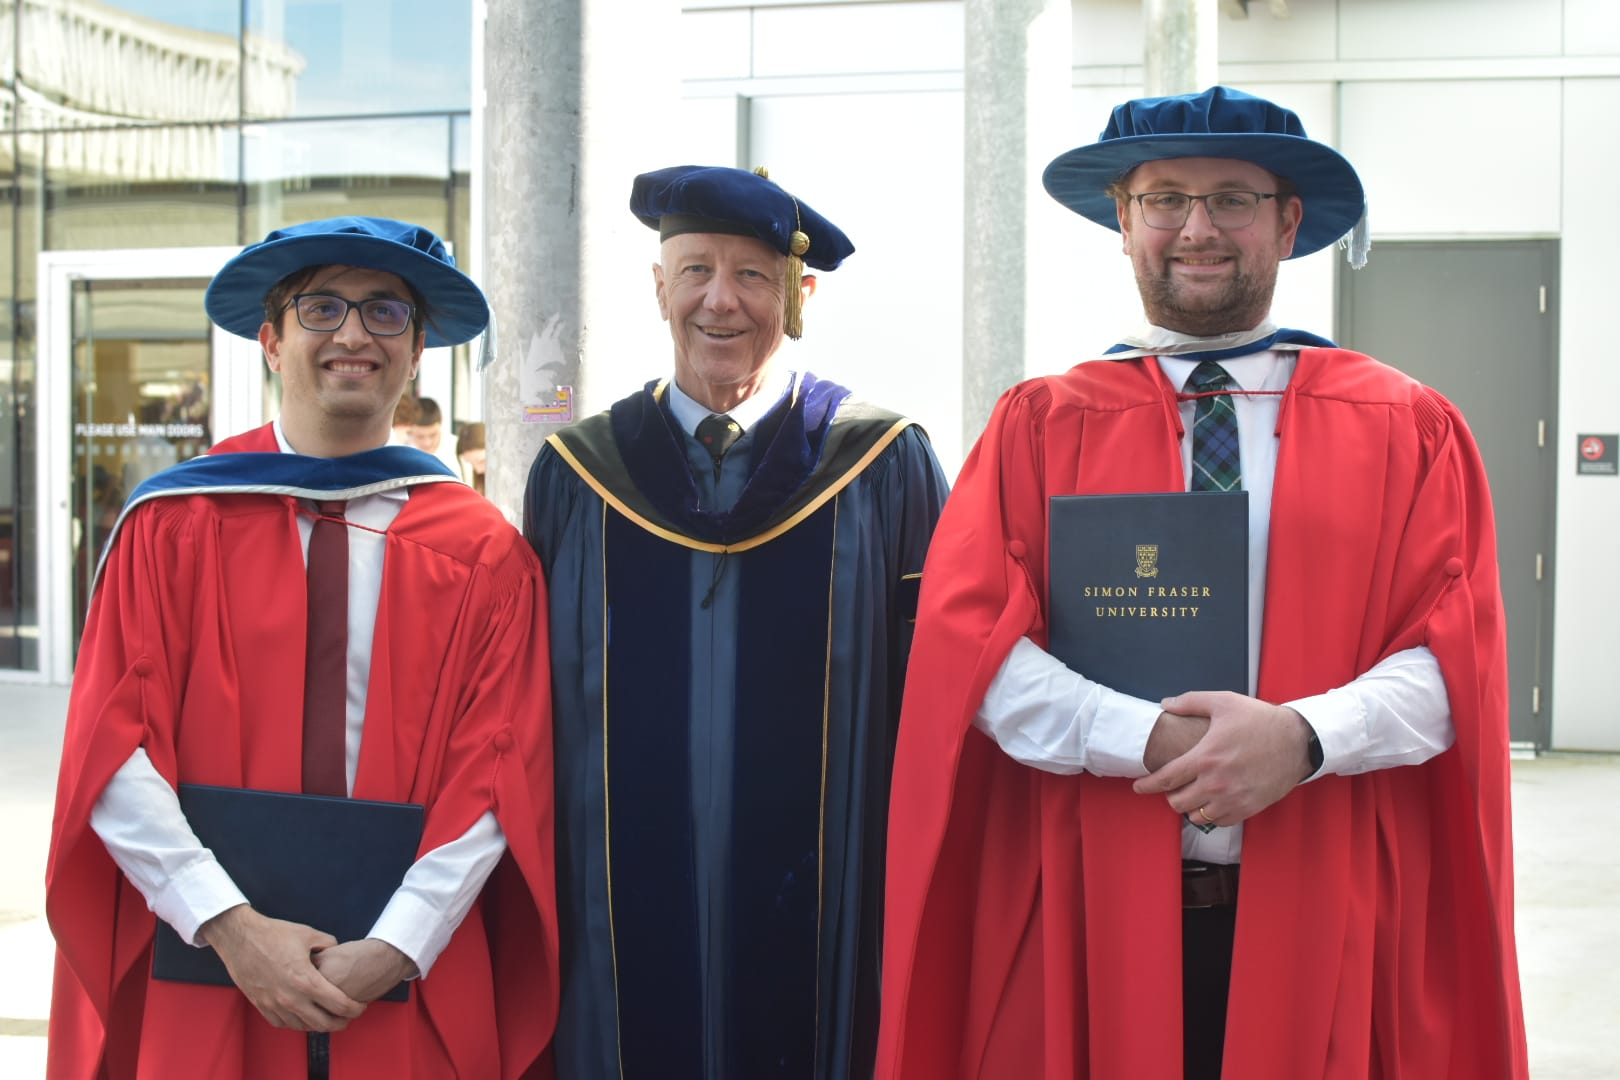
\includegraphics[width=\textwidth]{Figures/Convocation Image.jpg}
\end{frame}

\begin{frame}
    \centering
    \Huge Thank You
\end{frame}

\begin{frame}{Some References}
    \bibliographystyle{apalike}
    \bibliography{Refs}
\end{frame}

\end{document}
